\chapter{STRique Repeat Detection}
\label{sec:strique}

Expansions of short tandem repeats are genetic variants that have been implicated in several neuropsychiatric and other disorders, but their assessment remains challenging with current polymerase-based methods. Here we introduce a CRISPR-Cas-based enrichment strategy for nanopore sequencing combined with an algorithm for raw signal analysis. Our method, termed STRique for short tandem repeat identification, quantification and evaluation, integrates conventional sequence mapping of nanopore reads with raw signal alignment for the localization of repeat boundaries and a hidden Markov model-based repeat counting mechanism. We demonstrate the precise quantification of repeat numbers in conjunction with the determination of CpG methylation states in the repeat expansion and in adjacent regions at the single-molecule level without amplification. Our method enables the study of previously inaccessible genomic regions and their epigenetic marks.

\begin{figure}[h]
    \centering
    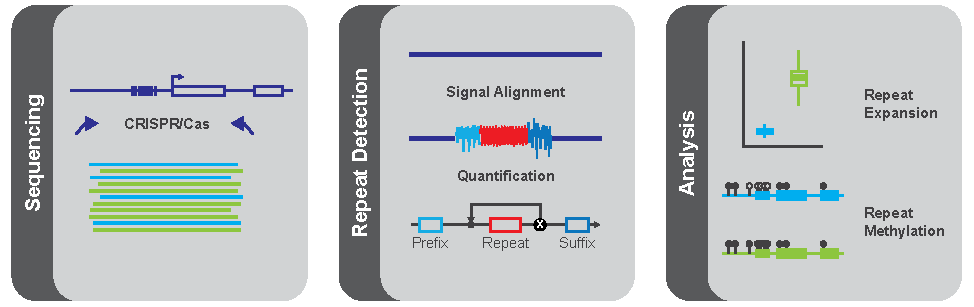
\includegraphics[width=1.0\textwidth]{figures/strique/GA.pdf}
    \label{fig:strique:ga}
\end{figure}




\section{Background}
\label{sec:strique:background}

The expansion of unstable genomic Short Tandem Repeats (STRs) causes more than 30 Mendelian human disorders.5 An extended GGGGCC-repeat $ [(G_{4}C_{2})_{n}] $ within the C9orf72 gene is the most frequent monogenic cause of Frontotemporal Dementia and Amyotrophic Lateral Sclerosis c9FTD/ALS.6 Similarly, accumulation of a CGG motif in the FMR1 gene underlies the Fragile X Syndrome, currently one of the most common identifiable genetic causes of mental retardation and autism.7 In both prototypical repeat expansion disorders, recent evidence has suggested pronounced inter- and intraindividual repeat variability as well as focal changes in DNA methylation to modulate the disease phenotype.8-10

To overcome current difficulties in characterizing expanded STRs we focused on three areas: i) optimization of nanopore sequencing and signal processing to capture STRs ii) development and implementation of a target enrichment strategy to increase efficiency and iii) integration of expansion measurements with CpG methylation at the single molecule level.
To enable a robust repeat analysis, we developed a general-purpose signal processing algorithm for the exact quantification of STR numbers in raw nanopore signals (STRique: Short Tandem Repeat identification, quantification \& evaluation, https://github.com/giesselmann/STRique). 


\section{Data Generation}
\label{sec:strique:data}



\section{Repeat Quantification}
\label{sec:strique:quantification}

\begin{figure}[h]
    \centering
    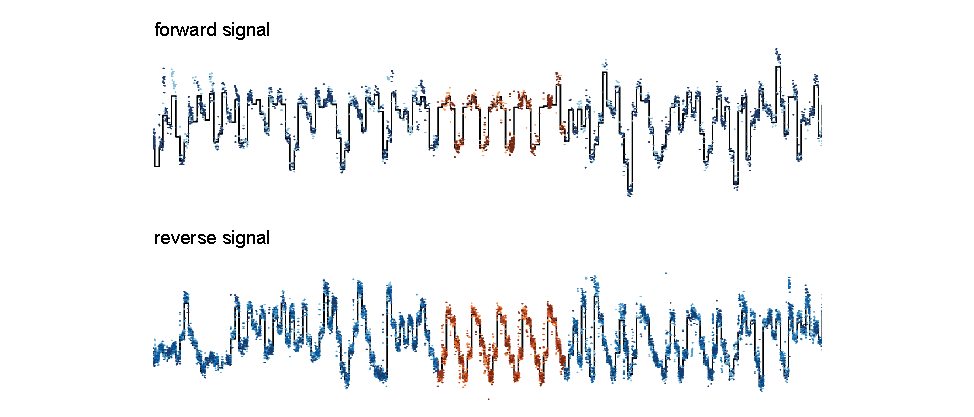
\includegraphics[width=1.0\textwidth]{figures/strique/signal.pdf}
    \captionsetup{format=plain}
    \caption[Nanopore raw signal of the C9orf72 STR in NA12878 cells]{Compound multi signal HMM alignment of publicly available raw traces from two template and eight complement reads from the NA12878 cell line shows matching signal pattern in all reads \cite{Jain2018}. Displayed are the current measurements as dots and the model signal as black line. Blue dots indicate current measurements identified as prefix or suffix sequence. Red dots indicate raw current measurements identified by STRique as belonging to the C9orf72-$ (G_{4}C_{2})_{n} $-STR. STRique detects in this case a $ (G_{4}C_{2})_{5} $-repeat.}
    \label{fig:strique:signal}
\end{figure}

\begin{figure}[h]
    \centering
    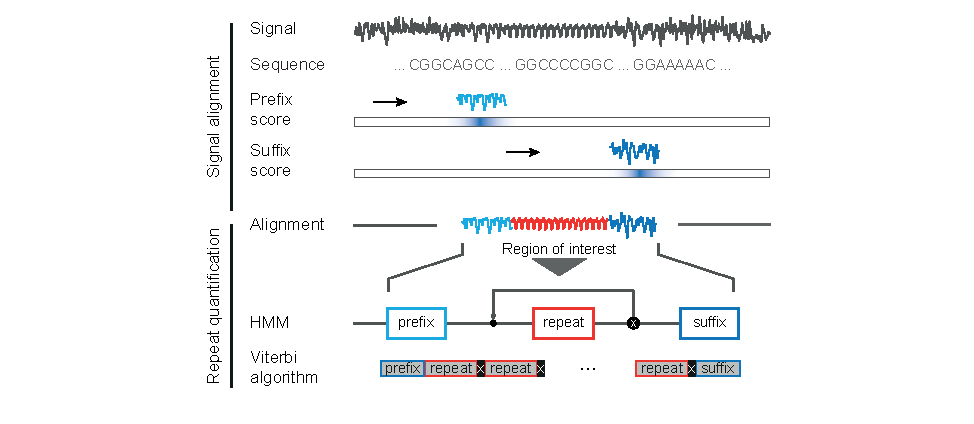
\includegraphics[width=1.0\textwidth]{figures/strique/count_structure_plasmid.pdf}
    \captionsetup{format=plain}
    \caption[STRique: generic repeat detection pipeline on raw nanopore signals.]{\textbf{a}, Repeat quantification enabled by raw signal alignment of flanking prefix and suffix regions and HMM-based count on the signal of interest. \textbf{b}, Bioanalyzer electropherogram, decoy alignment, RepeatHMM and STRique counts of synthetic $ (G_{4}C_{2})_{n} $ repeats.}
    \label{fig:strique:count_structure_plasmid}
\end{figure}

\begin{figure}[h]
    \centering
    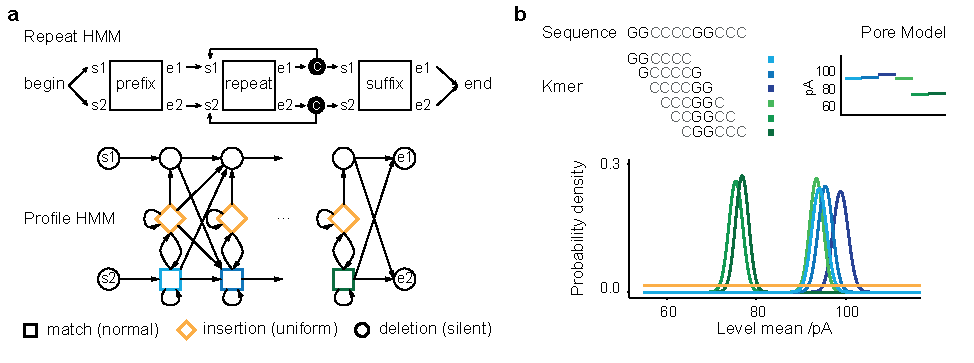
\includegraphics[width=1.0\textwidth]{figures/strique/count_hmm.pdf}
    \captionsetup{format=plain}
    \caption[Nanopore signal processing with STRique]{\textbf{a}, A compound profile HMM of prefix, a single repeat and the suffix sequence assigns either prefix, repeat or suffix label to each signal value. Repeat counts are obtained through dummy states between repeat and suffix. \textbf{b}, Nanopore signal profile HMM with normal distributed match state and uniform distributed insertion state emission probabilities.}
    \label{fig:strique:count_hmm}
\end{figure}

\begin{figure}[h]
    \centering
    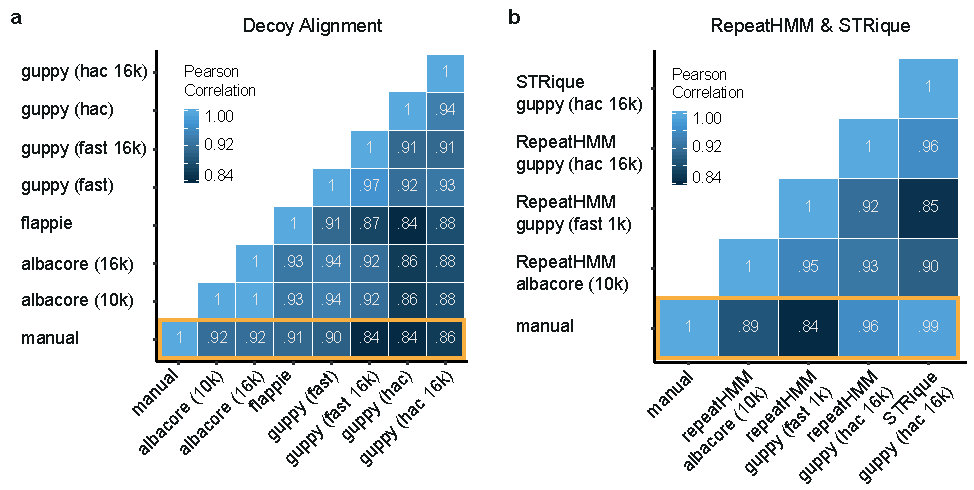
\includegraphics[width=1.0\textwidth]{figures/strique/count_sequence_corr.pdf}
    \captionsetup{format=plain}
    \caption[Correlation of sequence based STR detection methods]{\textbf{a}, Correlation of manual counted repeat lengths with sequence base methods. Decoy alignment against reference with 3-100 repeats with Albacore (window 10k and 16k), Guppy (fast and hac mode, 1k and 16k window size) and Flappie base-calling (n=204 reads). \textbf{b}, Correlation of manual count with RepeatHMM and STRique results (n=204 reads).}
    \label{fig:strique:count_sequence_corr}
\end{figure}

\begin{figure}[h]
    \centering
    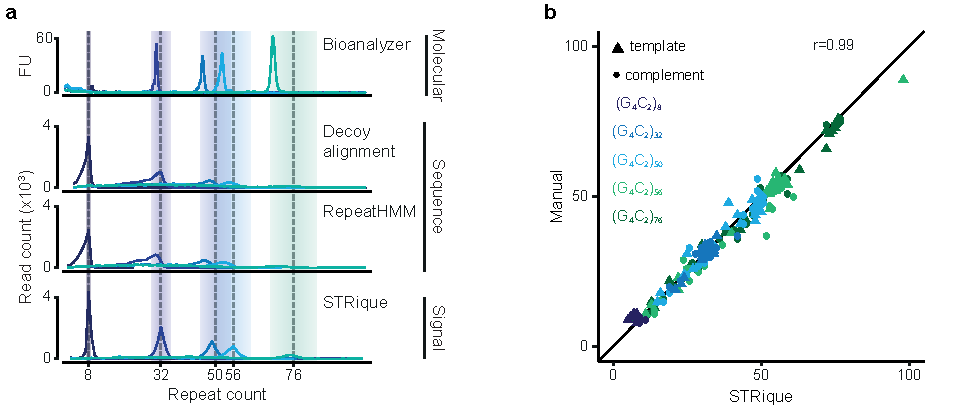
\includegraphics[width=1.0\textwidth]{figures/strique/count_signal_corr.pdf}
    \captionsetup{format=plain}
    \caption[Correlation and strand bias in STR analysis methods]{Manual counted set of plasmid reads on y-axis correlating with guppy base-calling and decoy alignment approach, RepeatHMM and STRique raw signal pipeline on x-axis. Only data points shown which could be evaluated with all four methods (n=15, 49, 45, 48, 47; Pearson correlation).}
    \label{fig:strique:count_signal_corr}
\end{figure}

\begin{figure}[h]
    \centering
    \includegraphics[width=1.0\textwidth]{figures/strique/count_bac.pdf}
    \captionsetup{format=plain}
    \caption[Strand bias in sequence based repeat counts]{Comparison of repeat counts from STRique, decoy alignment based on guppy (high accuracy model, 16k window size) and repeatHMM based on guppy (high accuracy model, 16k window size) for BAC data. One dot (n=5004) per read passing all three approaches and colored by strand.}
    \label{fig:strique:count_bac}
\end{figure}

\begin{figure}[h]
    \centering
    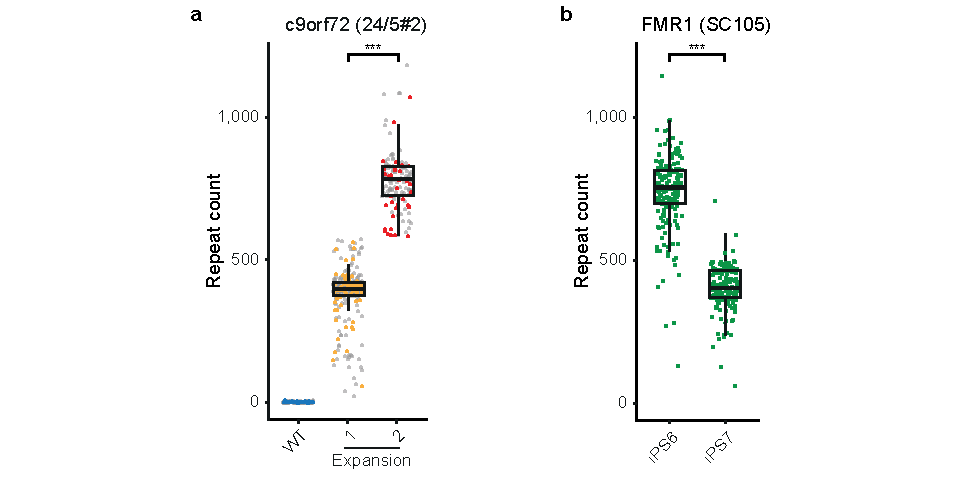
\includegraphics[width=1.0\textwidth]{figures/strique/count_patient_samples.pdf}
    \captionsetup{format=plain}
    \caption[Repeat quantification in c9orf72 and FMR1 patients]{\textbf{a}, Repeat quantification of sample 24/5\#2 at the C9orf72 locus, revealing two distinct repeat bands of ~450 and ~750 $ (G_{4}C_{2})_{n} $ repeats (n = 1,810, 738 and 363 evaluated reads with a difference in repeat length of 392 (95\% confidence interval (CI): 383 to 400), $ P < 2.2 \cdot 10^{-16} $). Colored points indicate reads used in Fig. \ref{fig:strique:methylation_c9orf72_region}b. WT, wild type. \textbf{b}, Repeat quantification of the SC105iPS6 and SC105iPS7 samples at the FMR1 locus (n = 174 and 168 evaluated reads with a difference in repeat length of -343 (95\% CI: -361 to -325), $ P < 2.2 \cdot 10^{-16} $). P values in a and b were obtained by a two-sided Wilcoxon rank-sum test; $ ***P < 0.001 $. Data are presented as boxplots (centerline, median; box limits, first and third quartiles; whiskers, 1.5x interquartile range).}
    \label{fig:strique:count_patients}
\end{figure}

\begin{figure}[h]
    \centering
    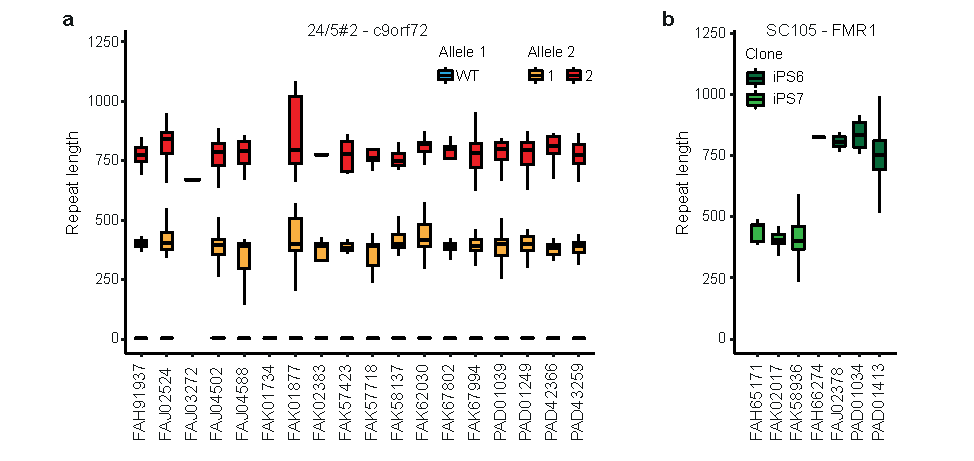
\includegraphics[width=1.0\textwidth]{figures/strique/count_experiments.pdf}
    \captionsetup{format=plain}
    \caption[Repeat count cluster stability over experiments]{\textbf{a}, C9orf72 target enrichment flow cells for patient 24/5\#2 \textbf{b}, FMR1 enrichment flow cells of SC105iPS6/iPS7. (FA*: MinION, PAD*: PromethION, number of reads per boxplot are in Supplementary Tables 5-6 column wt and exp). Data presented as boxplots (centerline, median; box limits, first and third quartiles; whiskers, 1.5x interquartile range; outliers not shown)}
    \label{fig:strique:count_experiments}
\end{figure}




\section{Base Modification Detection}
\label{sec:strique:modifications}

\begin{figure}[h]
    \centering
    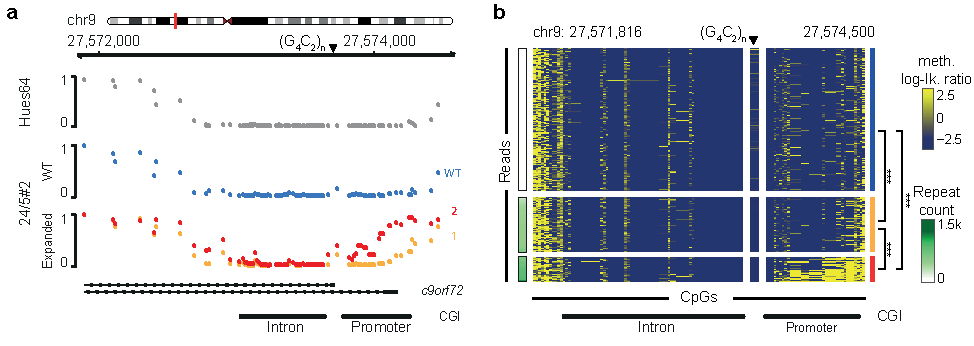
\includegraphics[width=1.0\textwidth]{figures/strique/methylation_c9orf72_region.pdf}
    \captionsetup{format=plain}
    \caption[Methylation state analyses at the single-read level]{\textbf{a}, C9orf72 methylation status in HUES64 as measured by whole-genome bisulfite sequencing. The wild-type (blue) allele and expanded (ex; orange) alleles (with 450 and 750 $ (G_{4}C_{2})_{n} $ repeats (red), respectively) are shown for patient 24/5\#2, as measured by nanopore sequencing. \textbf{b}, Single read nanopore methylation of C9orf72 covering reads from the minus strand (n = 259, 100 and 43 rows per block) sorted by detected repeat length (rows, single read; columns, single CpGs). CpGs with logP ratio $> 2.5$ are considered methylated, while those with logP ratio $< -2.5$ are considered unmethylated. The median methylation difference (95\% CI) and P value (determined by two-sided Wilcoxon rank-sum test on mean promoter CGI methylation) for comparisons were as follows: $ WT-ex450: 3.9 \cdot 10^{-5} (4.8 \cdot 10^{-6} to 3.4 \cdot 10^{-2}), P = 5.3 \cdot 10^{-9}; WT-ex750: 0.56 (0.46-0.64), P < 2.2 \cdot 10^{-16}; ex450-ex750: 0.53 (0.40-0.64), P < 2.2 \cdot 10^{-16}; ***P < 0.001. $ }
    \label{fig:strique:methylation_c9orf72_region}
\end{figure}

\begin{figure}[h]
    \centering
    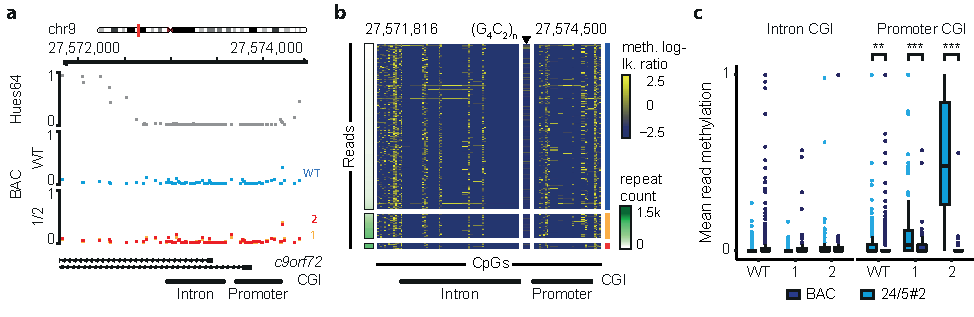
\includegraphics[width=1.0\textwidth]{figures/strique/methylation_bac_region.pdf}
    \captionsetup{format=plain}
    \caption[Nanopore single read methylation in BAC data]{\textbf{a}, Methylation status of c9orf72 region in BAC data for repeats < 200 (WT), 200-750 (Cluster1,orange) and > 750 (Cluster2,red) and control (Hues64, WGBS) \textbf{b}, Single read methylation on a sample of 500 BAC minus strand reads sorted by repeat count (row split 200 and 750 repeats, n=423,63,14). \textbf{c}, Difference in mean CGI methylation of intron and promoter per read on minus strand. Reads binned by detected repeat length for BAC (n=2066 WT; 315 Cluster1; 72 Cluster2) and patient 24/5\#2 (n=925 WT; 362 Cluster1; 153 Cluster2). Two sided Wilcoxon rank sum test, corrected for multiple testing (Holm), q-vals: * 0.05 - 0.01; ** 0.01 - 0.001; *** < 0.001. Median methylation differences between promoter CGI [95\%CI] for WT $-2.3e^{-5} [CI: -5.6e^{-6}:-1.5e^{-5}, q=7.4e^{-3}] $ and Cluster1 $ -0.01 [CI: -7.1e^{-5}:-3.4e^{-2}, q=1.4e^{-17}] $ and Cluster2 $ -0.46 [CI: -0.58:-0.37, q=1.0e^{-26}] $.}
    \label{fig:strique:methylation_bac_region}
\end{figure}

\begin{figure}[h]
    \centering
    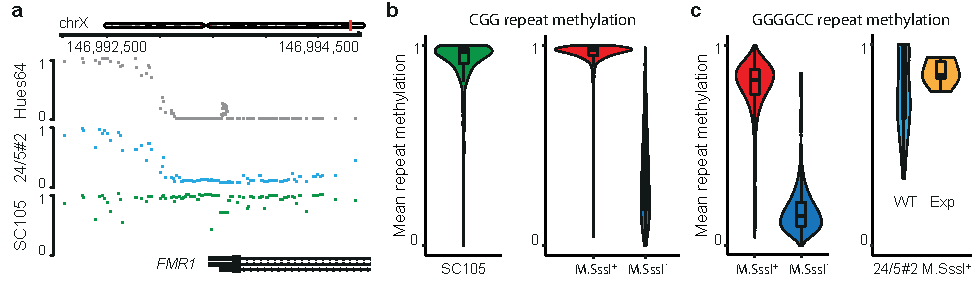
\includegraphics[width=1.0\textwidth]{figures/strique/methylation_repeat.pdf}
    \captionsetup{format=plain}
    \caption[Region and repeat methylation detection]{\textbf{a}, FMR1 region methylation in SC105iPS6/iPS7 compared to Hues64 WGBS and patient sample 24/5\#2. \textbf{b}, CGG mean repeat methylation status detected by STRique for SC105 (n=197) and synthetic plasmid control with 99 repeats treated with $ M.SssI^{+/-} $ (5mC level on minus strand, n=1232 $ M.SssI^{+} $; n=11991 $ M.SssI^{-} $). \textbf{c}, GGGGCC repeat methylation status for plasmid control with 76 repeats treated with $ M.SssI^{+/-} $ (n=2939 $ M.SssI^{+} $; n=31280 $ M.SssI^{-} $) and patient sample 24/5\#2 treated with $ M.SssI^{+} $ (5mC level on minus strand, n=52 WT and n=6 Cluster1). Data in (b-c) presented as violin plots with overlayed boxplots (centerline, median; box limits, first and third quartiles; whiskers, 1.5x interquartile range; outliers not shown).}
    \label{fig:strique:methylation_repeat}
\end{figure}




\section{Summary}
\label{sec:strique:summary}




